\documentclass[11pt]{article}

\usepackage{fullpage}
\usepackage{amsmath, amssymb, bm, cite, epsfig, psfrag}
\usepackage{graphicx}
\usepackage{float}
\usepackage{amsthm}
\usepackage{amsfonts}
\usepackage{listings}
\usepackage{cite}
\usepackage{hyperref}
\usepackage{tikz}
\usepackage{enumerate}
\usepackage[outercaption]{sidecap}
\usetikzlibrary{shapes,arrows}
%\usetikzlibrary{dsp,chains}

%\restylefloat{figure}
%\theoremstyle{plain}      \newtheorem{theorem}{Theorem}
%\theoremstyle{definition} \newtheorem{definition}{Definition}

\def\del{\partial}
\def\ds{\displaystyle}
\def\ts{\textstyle}
\def\beq{\begin{equation}}
\def\eeq{\end{equation}}
\def\beqa{\begin{eqnarray}}
\def\eeqa{\end{eqnarray}}
\def\beqan{\begin{eqnarray*}}
\def\eeqan{\end{eqnarray*}}
\def\nn{\nonumber}
\def\binomial{\mathop{\mathrm{binomial}}}
\def\half{{\ts\frac{1}{2}}}
\def\Half{{\frac{1}{2}}}
\def\N{{\mathbb{N}}}
\def\Z{{\mathbb{Z}}}
\def\Q{{\mathbb{Q}}}
\def\R{{\mathbb{R}}}
\def\C{{\mathbb{C}}}
\def\argmin{\mathop{\mathrm{arg\,min}}}
\def\argmax{\mathop{\mathrm{arg\,max}}}
%\def\span{\mathop{\mathrm{span}}}
\def\diag{\mathop{\mathrm{diag}}}
\def\x{\times}
\def\limn{\lim_{n \rightarrow \infty}}
\def\liminfn{\liminf_{n \rightarrow \infty}}
\def\limsupn{\limsup_{n \rightarrow \infty}}
\def\GV{Guo and Verd{\'u}}
\def\MID{\,|\,}
\def\MIDD{\,;\,}

\newtheorem{proposition}{Proposition}
\newtheorem{definition}{Definition}
\newtheorem{theorem}{Theorem}
\newtheorem{lemma}{Lemma}
\newtheorem{corollary}{Corollary}
\newtheorem{assumption}{Assumption}
\newtheorem{claim}{Claim}
\def\qed{\mbox{} \hfill $\Box$}
\setlength{\unitlength}{1mm}

\def\bhat{\widehat{b}}
\def\ehat{\widehat{e}}
\def\phat{\widehat{p}}
\def\qhat{\widehat{q}}
\def\rhat{\widehat{r}}
\def\shat{\widehat{s}}
\def\uhat{\widehat{u}}
\def\ubar{\overline{u}}
\def\vhat{\widehat{v}}
\def\xhat{\widehat{x}}
\def\xbar{\overline{x}}
\def\zhat{\widehat{z}}
\def\zbar{\overline{z}}
\def\la{\leftarrow}
\def\ra{\rightarrow}
\def\MSE{\mbox{\small \sffamily MSE}}
\def\SNR{\mbox{\small \sffamily SNR}}
\def\SINR{\mbox{\small \sffamily SINR}}
\def\arr{\rightarrow}
\def\Exp{\mathbb{E}}
\def\var{\mbox{var}}
\def\Tr{\mbox{Tr}}
\def\tm1{t\! - \! 1}
\def\tp1{t\! + \! 1}

\def\Xset{{\cal X}}

\newcommand{\one}{\mathbf{1}}
\newcommand{\abf}{\mathbf{a}}
\newcommand{\bbf}{\mathbf{b}}
\newcommand{\dbf}{\mathbf{d}}
\newcommand{\ebf}{\mathbf{e}}
\newcommand{\gbf}{\mathbf{g}}
\newcommand{\hbf}{\mathbf{h}}
\newcommand{\pbf}{\mathbf{p}}
\newcommand{\pbfhat}{\widehat{\mathbf{p}}}
\newcommand{\qbf}{\mathbf{q}}
\newcommand{\qbfhat}{\widehat{\mathbf{q}}}
\newcommand{\rbf}{\mathbf{r}}
\newcommand{\rbfhat}{\widehat{\mathbf{r}}}
\newcommand{\sbf}{\mathbf{s}}
\newcommand{\sbfhat}{\widehat{\mathbf{s}}}
\newcommand{\ubf}{\mathbf{u}}
\newcommand{\ubfhat}{\widehat{\mathbf{u}}}
\newcommand{\utildebf}{\tilde{\mathbf{u}}}
\newcommand{\vbf}{\mathbf{v}}
\newcommand{\vbfhat}{\widehat{\mathbf{v}}}
\newcommand{\wbf}{\mathbf{w}}
\newcommand{\wbfhat}{\widehat{\mathbf{w}}}
\newcommand{\xbf}{\mathbf{x}}
\newcommand{\xbfhat}{\widehat{\mathbf{x}}}
\newcommand{\xbfbar}{\overline{\mathbf{x}}}
\newcommand{\ybf}{\mathbf{y}}
\newcommand{\zbf}{\mathbf{z}}
\newcommand{\zbfbar}{\overline{\mathbf{z}}}
\newcommand{\zbfhat}{\widehat{\mathbf{z}}}
\newcommand{\Ahat}{\widehat{A}}
\newcommand{\Abf}{\mathbf{A}}
\newcommand{\Bbf}{\mathbf{B}}
\newcommand{\Cbf}{\mathbf{C}}
\newcommand{\Bbfhat}{\widehat{\mathbf{B}}}
\newcommand{\Dbf}{\mathbf{D}}
\newcommand{\Gbf}{\mathbf{G}}
\newcommand{\Hbf}{\mathbf{H}}
\newcommand{\Kbf}{\mathbf{K}}
\newcommand{\Pbf}{\mathbf{P}}
\newcommand{\Phat}{\widehat{P}}
\newcommand{\Qbf}{\mathbf{Q}}
\newcommand{\Rbf}{\mathbf{R}}
\newcommand{\Rhat}{\widehat{R}}
\newcommand{\Sbf}{\mathbf{S}}
\newcommand{\Ubf}{\mathbf{U}}
\newcommand{\Vbf}{\mathbf{V}}
\newcommand{\Wbf}{\mathbf{W}}
\newcommand{\Xhat}{\widehat{X}}
\newcommand{\Xbf}{\mathbf{X}}
\newcommand{\Ybf}{\mathbf{Y}}
\newcommand{\Zbf}{\mathbf{Z}}
\newcommand{\Zhat}{\widehat{Z}}
\newcommand{\Zbfhat}{\widehat{\mathbf{Z}}}
\def\alphabf{{\boldsymbol \alpha}}
\def\betabf{{\boldsymbol \beta}}
\def\mubf{{\boldsymbol \mu}}
\def\lambdabf{{\boldsymbol \lambda}}
\def\etabf{{\boldsymbol \eta}}
\def\xibf{{\boldsymbol \xi}}
\def\taubf{{\boldsymbol \tau}}
\def\sigmahat{{\widehat{\sigma}}}
\def\thetabf{{\bm{\theta}}}
\def\thetabfhat{{\widehat{\bm{\theta}}}}
\def\thetahat{{\widehat{\theta}}}
\def\mubar{\overline{\mu}}
\def\muavg{\mu}
\def\sigbf{\bm{\sigma}}
\def\etal{\emph{et al.}}
\def\Ggothic{\mathfrak{G}}
\def\Pset{{\mathcal P}}
\newcommand{\bigCond}[2]{\bigl({#1} \!\bigm\vert\! {#2} \bigr)}
\newcommand{\BigCond}[2]{\Bigl({#1} \!\Bigm\vert\! {#2} \Bigr)}

\def\Rect{\mathop{Rect}}
\def\sinc{\mathop{sinc}}
\def\Real{\mathrm{Re}}
\def\Imag{\mathrm{Im}}



\begin{document}

\title{Problems:  RX Filtering}
\author{Prof.\ Sundeep Rangan}
\date{}

\maketitle

\begin{enumerate}

\item \emph{Effective discrete-time channel.}
Consider a digital transmission and reception performed in the following steps:
\begin{align} \label{eq:txrx}
\begin{split}
    u(t) &= \sum s[n] p_{tx}(t-nT), \\
    y(t) &= h_{\rm chan}(t) * u(t) \\
    r[n] &= v(nT), \quad v(t) = p_{\rm rx}(t) * y(t)
\end{split}
\end{align}
Suppose that
\[
    p_{\rm rx}(t) = p_{\rm tx}(t) = \frac{1}{\sqrt{T}}\mathrm{sinc}(t/T),
\]
and
\[
    h_{\rm chan}(t) = G_1 \delta(t-\tau_1) + G_2 \delta(t-\tau_2).
\]
\begin{enumerate}[(a)]
\item Find $g(t) = p_{\rm rx}(t)*p_{\rm tx}(t)*h_{\rm chan}(t)$,
the channel impulse response with filtering.
\item Find the effective discrete-time impulse response, $h[n]$,
such that
\[
    r[n] = \sum_k h[k]s[n-k].
\]
\item Use MATLAB to plot $h[k]$ when $G_1=1$, $G_2=0.1$,
$\tau_1 = 0$,  $\tau_2 = 20$ ns and $1/T=$ 1 GHz.
\end{enumerate}

\item \emph{Compute a time-domain response}:
Consider a digital transmission and reception performed in the  steps
in \eqref{eq:txrx} with
\[
    p_{\rm rx}(t) = \delta(t), \quad p_{\rm tx}(t) = \delta(t-\tau),
\]
and
\[
    \frac{dy(t)}{dt} = \frac{a}{T}(u(t) - y(t)),
\]
for some $a> 0$.
\begin{enumerate}[(a)]
\item Find $h_{\rm chan}(t)$, the baseband impulse response from $u(t)$ to $y(t)$.
\item Find $g(t)=p_{\rm rx}(t)*p_{tx}(t)*h_{\rm chan}(t)$, the baseband impulse
response with filtering.
\item Use MATLAB to plot $h[n]$ the effective discrete-time channel response when $\tau=3.5 T$,
$a=0.1$.
\item Use MATLAB to plot the response $r[n]$ when
\[
    s[n] = \begin{cases}
        1 & n =0,1,\ldots,9 \\
        0 & \mbox{else.}
    \end{cases}
\]
\end{enumerate}


\begin{figure}
\center
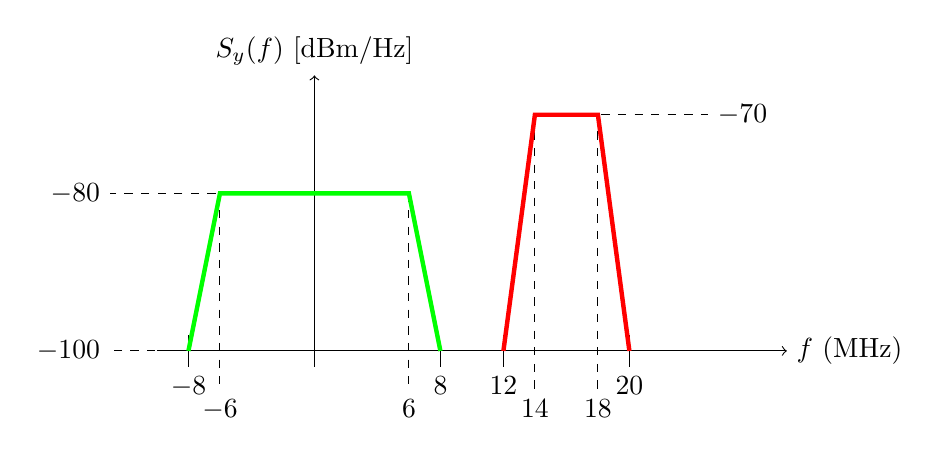
\begin{tikzpicture}[xscale=2,yscale=1]
    \pgfmathsetmacro{\fa}{0.6}
    \pgfmathsetmacro{\fb}{0.8}
    \pgfmathsetmacro{\fc}{1.2}
    \pgfmathsetmacro{\fd}{1.4}
    \pgfmathsetmacro{\fe}{1.8}
    \pgfmathsetmacro{\ff}{2.0}
    \pgfmathsetmacro{\fm}{3}
    \pgfmathsetmacro{\Sa}{2}
    \pgfmathsetmacro{\Sb}{3}
    \pgfmathsetmacro{\tic}{0.2}
    \pgfmathsetmacro{\ticb}{0.5}
    % Draw the axes
    \draw [->] (-1,0) -- (3,0) node [right] {$f$ (MHz)};
    \draw [->] (0,-\tic) -- (0,3.5) node [above] {$S_y(f)$ [dBm/Hz]};

    % x-axis labels
    \draw [-] (-\fb,\tic) -- (-\fb,-\tic) node [below] {$-8$};
    \draw [-,dashed] (-\fa,\Sa) -- (-\fa,-\ticb) node [below] {$-6$};
    \draw [-,dashed] (\fa,\Sa) -- (\fa,-\ticb) node [below] {$6$};
    \draw [-] (\fb,0) -- (\fb,-\tic) node [below] {$8$};
    \draw [-] (\fc,\tic) -- (\fc,-\tic) node [below] {$12$};
    \draw [-,dashed] (\fd,\Sb) -- (\fd,-\ticb) node [below] {$14$};
    \draw [-,dashed] (\fe,\Sb) -- (\fe,-\ticb) node [below] {$18$};
    \draw [-] (\ff,\tic) -- (\ff,-\tic) node [below] {$20$};

    % y-axis labels
    \draw [-,dashed] (-\fa+0.5,\Sa) -- (-1.3,\Sa) node [left] {$-80$};
    \draw [-,dashed] (\fd,\Sb) -- (2.5,\Sb) node [right] {$-70$};
    \draw [-,dashed] (-\fb,0) -- (-1.3,0) node [left] {$-100$};


    % Draw PSD S_u(\Omega)
    \draw [ultra thick,green,-] (-\fb,0) -- (-\fa,\Sa) -- (\fa,\Sa) -- (\fb,0);
    \draw [ultra thick,red,-] (\fc,0) -- (\fd,\Sb) -- (\fe,\Sb) -- (\ff,0);
\end{tikzpicture}

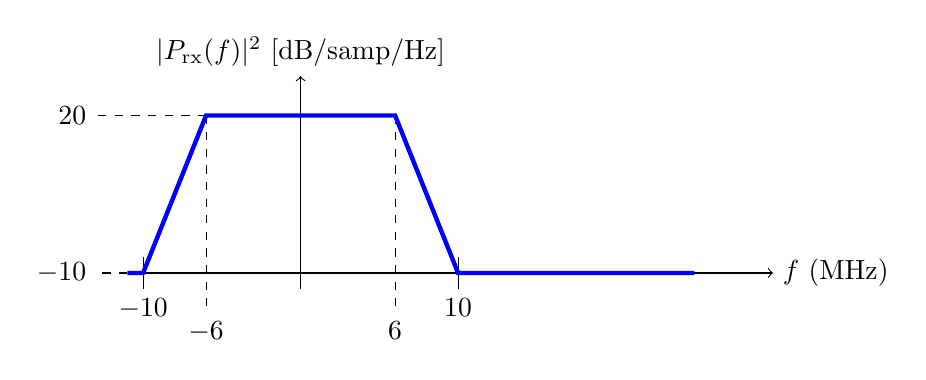
\begin{tikzpicture}[xscale=2,yscale=1]
    \pgfmathsetmacro{\tic}{0.2}
    \pgfmathsetmacro{\ticb}{0.5}
    % Draw the axes
    \draw [->] (-1,0) -- (3,0) node [right] {$f$ (MHz)};
    \draw [->] (0,-\tic) -- (0,2.5) node [above] {$|P_{\rm rx}(f)|^2$ [dB/samp/Hz]};

    % x-axis labels
    \draw [-] (-1,\tic) -- (-1,-\tic) node [below] {$-10$};
    \draw [-,dashed] (-0.6,2) -- (-0.6,-\ticb) node [below] {$-6$};
    \draw [-,dashed] (0.6,2) -- (0.6,-\ticb) node [below] {$6$};
    \draw [-] (1,\tic) -- (1,-\tic) node [below] {$10$};

    % y-axis labels
    \draw [-,dashed] (-0.6,2) -- (-1.3,2) node [left] {$20$};
    \draw [-,dashed] (-1.1,0) -- (-1.3,0) node [left] {$-10$};

    % Draw PSD S_u(\Omega)
    \draw [ultra thick,blue,-] (-1.1,0)--(-1,0) -- (-0.6,2) -- (0.6,2) -- (1,0) -- (2.5,0);
\end{tikzpicture}

\caption{Figures for Problem~\ref{prob:rxpsd}.  Top:
PSD of the input the RX filter $y(t)$.  Bottom:  RX filter frequency response.
}
\label{fig:rxpsd}
\end{figure}

\item  \emph{Sampling in frequency-domain}.  Suppose that $v(t)$ has a Fourier Transform,
\[
    V(f) = \begin{cases}
                \sqrt{C} & \mbox{if } f \in [0,10] \mbox{ MHz} \\
                0 & \mbox{else },
            \end{cases}
\]
where $C = 5(10)^{-6}$ mJ/Hz.
\begin{enumerate}[(a)]
\item What is the energy of the signal in dBmJ?
\item Find $v(t)$.
\item If $r[n] = v(nT)$ with $1/T = 15$ MHz, draw $R(\Omega)$.
\end{enumerate}

\item \label{prob:rxpsd}  \emph{RX PSD.}  A received signal $y(t)$ has two components with PSD shown
in the top of Fig.~\ref{fig:rxpsd}:  A desired signal (green) and interfering signal (red).
The signal is filtered $v(t) = p_{\rm rx}(t) * y(t)$ with the frequency response 
in the bottom panel of Fig.~\ref{fig:rxpsd}.
\begin{enumerate}
\item Draw the PSD, $S_v(f)$, of the filtered signal $v(t)$.  
The units of $S_v(f)$ is dBm/Hz$^2$/sample.  

\item Draw the discrete-time PSD of the sampled signal $r[n] = v(nT)$ for a sample rate
$\frac{1}{T}=40$ MHz.

\item  For the component of the signal $y(t)$ with $|f|\leq 6$~MHz, what is the energy
per sample in $r[n]$?  State your answer in dBmJ/sample.

\end{enumerate}

\end{enumerate}

\end{document}
